\documentclass{beamer}
\usepackage[french]{babel}
\usepackage{hyperref}
\definecolor{links}{HTML}{2A1B81}
\hypersetup{colorlinks,linkcolor=,urlcolor=links}
\usepackage{graphicx}
\usepackage{amsmath,amssymb}
\usepackage{tabularx}
\usepackage{booktabs}
\usepackage[compatibility=false]{caption}
\usepackage[toc,page]{appendix}
\usepackage{minted}
\usepackage{xspace}

\makeatletter
  \def\beamer@calltheme#1#2#3{%
    \def\beamer@themelist{#2}
    \@for\beamer@themename:=\beamer@themelist\do
    {\usepackage[{#1}]{\beamer@themelocation/#3\beamer@themename}}}

  \def\usefolder#1{
    \def\beamer@themelocation{#1}
  }
  \def\beamer@themelocation{}

\patchcmd{\minted@colorbg}{\noindent}{\medskip\noindent}{}{}
\apptocmd{\endminted@colorbg}{\par\medskip}{}{}
\makeatother

\newcolumntype{Y}{>{\centering\arraybackslash}X}

\usefolder{../theme}
\usetheme[numbering=fraction,block=fill,progressbar=frametitle]{metropolis} %Use metropolis theme

\definecolor{bg}{rgb}{0.95,0.95,0.95}
\setminted{bgcolor=bg,fontsize=\scriptsize,autogobble,mathescape,breaklines,tabsize=2}
\setmintedinline{breaklines,autogobble,fontsize=\scriptsize}
\setbeamersize{text margin left=8pt,text margin right=8pt}
\setbeamercovered{transparent}

\begin{document}

\title[C++]{Introduction à la programmation en C++}
\author[nicolas.audebert@onera.fr]{Nicolas Audebert}
\setmainfont{Fira Sans}


\AtBeginSection[]{
  \begin{frame}{Plan de la séance}
  \small \tableofcontents[currentsection]
  \end{frame}
}

\newcommand\cppi[1]{\mintinline{cpp}{#1}}
\newcommand\cpp[1]{%
  \begin{minted}{cpp}
  #1
  \end{minted}
}%

\author[nicolas.audebert@onera.fr]{Nicolas Audebert}
\date[1 déc. 2017]{Vendredi 1\textsuperscript{er} décembre 2017}
\subtitle{Chaînes de caractères - Fichiers}
\maketitle

\begin{frame}{Avant toute chose}
  \begin{alertblock}{Rendus de TP et des exercices}
  Les rendus se font sur \href{https://educnet.enpc.fr}{\textbf{Educnet}}, même en cas de retard. \textbf{Pas par mail}.
  \begin{enumerate}
  	\item Le code rendu \textbf{doit compiler}.
    \item Le code rendu doit \textbf{être propre} (indentation, noms de variables clairs).
    \item Le code rendu doit \textbf{être commenté} (réponses aux questions, fonctionnement du code).
    \item Rassembler le code dans une seule archive (\texttt{.zip}, \texttt{.rar}, \texttt{.tar.gz}, etc.).
  \end{enumerate}
  Un exercice ou un TP rendu en retard ou ne respectant pas une des consignes ci-dessus sera pénalisé.
  \end{alertblock}
\end{frame}

\section{À propos du partiel}

\begin{frame}[fragile]{Quizz 1}

Que fait ce code ?

\begin{minted}{cpp}
bool paire(Main m){
    bool res = false;
    for(int i=0; i<5; i++){
        for(int j=i; j<5; j++){
            if(m.cartes[i] == m.cartes[j]){
                res = true;
            }
        }
    }
}

bool test = paire();
\end{minted}

\only<2>
{Il renvoie toujours la même chose, indépendant de \texttt{m}. En effet, on a oublié d'ajouter \texttt{return res;} à la fin de la fonction\dots}
\end{frame}

\begin{frame}[fragile]{Quizz 2}

Que fait ce code ?

\begin{minted}{cpp}
Carte c = {VALET, COEUR};
Main m;
...
for(int i=0; i<5; i++){
    if(m.cartes[i] = c){
        cout << "Valet de coeur" << endl;
    }
}
\end{minted}

\only<2>
{Il change la valeur de toutes les cartes de la main pour les remplacer par le Valet de c\oe{}ur. En effet, on a confondu l'opérateur d'affectation (\texttt{=}) et l'opérateur d'égalité (\texttt{==}).}
\end{frame}

\begin{frame}[fragile]{Quizz 3}

Peut-on raccourcir ce code ?

\begin{minted}{cpp}
bool ma_fonction(bool test1, bool test2){
    bool result;
    if((test1 && test2) == true){
        result = false;
    } else {
        result = true;
    }
    return result;
}
\end{minted}

\begin{overprint}
\onslide<1>
{}
\onslide<2>
\begin{minted}{cpp}
// Oui ! Il faut manipuler directement le booléen.
bool ma_fonction(bool test1, bool test2){
   return !(test1 && test2);
}
\end{minted}
\end{overprint}
\end{frame}

\begin{frame}[fragile]{Quizz 4}
Que fait ce code ?

\begin{minted}{cpp}
int tab[1000];

for(int i=0; i<1000; i++){
    if(i%2 == 0)
        cout << i << " est paire" << endl;
        cout << "Sa moitié est " << i/2 << endl;
    
    tab[i] = i;
}
\end{minted}

\only<2>
{Si le nombre est pair, il affiche "n est paire". Dans tous les cas, il affiche la moitié du nombre. En effet, sans accolades, le \texttt{if} ne porte que sur l'instruction suivante. L'indentation ici est trompeuse !}
\end{frame}

\begin{frame}[fragile]{Quizz 5}
Que fait ce code ?

\begin{minted}{cpp}
void remplitCarte(Carte c){
	// on remplit une carte aléatoirement
    c.valeur = rand()%13 + 2;
    c.couleur = rand()%4;
}

Carte c;
remplitCarte(c);
cout << c.valeur << ", " << c.couleur << endl;
\end{minted}

\only<2>
{\texttt{c} a des valeurs aléatoires. En effet, la fonction \texttt{remplitCarte} ne fait que modifier une copie de la carte passée en argument. Il fallait la passer par référence\dots}
\end{frame}


\begin{frame}{Conseils}

\begin{itemize}
	\item Bien \textbf{réviser} les bases: passage par valeur, passage par référence, manipulation des booléens, manipulation des tableaux
    \item \textbf{Tester son code} régulièrement et lire attentivement les erreurs de compilation.
    \item Ne pas hésiter à \textbf{afficher le contenu des variables} avec \texttt{cout} pour comprendre ce qui se passe.
    \item \textbf{Indenter} correctement son code et ne pas oublier les accolades.
    \item Mettre des \textbf{commentaires}, pour soi et pour le correcteur.
\end{itemize}
\end{frame}

\section{Rappels}
\begin{frame}[fragile]{Notion de constructeur}
    \only<1>{L'initialisation d'un objet fait appel au \textbf{constructeur} de sa classe.}

    \begin{block}{Définition}
      Un \textbf{constructeur} est une méthode\,:
      \begin{itemize}
          \item qui \textbf{n'a pas} de type de retour,
          \item qui porte \textbf{le même nom} que la classe,
          \item qui décrit comment initialiser les instances de la classe.
      \end{itemize}
    \end{block}
    \begin{overprint}
    \onslide<1>
    \begin{alertblock}{Manipulation}
      Un constructeur :
      \begin{itemize}
          \item est \textbf{systématiquement} appelé à la création d'un objet,
          \item ne peut pas être appelé \textbf{après} la création de l'objet.
      \end{itemize}
    \end{alertblock}

    \onslide<2>
    \begin{minipage}{\linewidth}
    \begin{minipage}{0.59\linewidth}
            \begin{minted}{cpp}
class Point{
    double x,y;
public:
    Point(double valX, double valY);
    ...
}

// Définition du constructeur
Point::Point(double valX, double valY){
    x = valX; y = valY;
}
            \end{minted}
    \end{minipage}
    \hfill
    \begin{minipage}{0.39\linewidth}
            \begin{minted}{cpp}
...
Point b = {2,3}; // ERREUR
Point c(2,3); // OK
// Cette syntaxe appelle
// le constructeur
            \end{minted}
        
    \end{minipage}
    \end{minipage}
    \end{overprint}
\end{frame}

\begin{frame}[fragile=singleslide]{Le constructeur vide}
    À la création de l'objet il y a \textbf{toujours} un appel à un constructeur.

    Lorsqu'aucun constructeur n'est défini par l'utilisateur, le compilateur en créé un par défaut.
    C'est un \textbf{constructeur vide} qui ne prend aucun argument et ne fait que créer les champs de l'objet.
        \begin{minted}{cpp}
class Point{
    double x,y;
public:
    double get(double& x, double& y);
    void set(double valX, double valY);
};
...
Point a;// Appel au constructeur par défaut
        \end{minted}
    
\end{frame}


\begin{frame}[fragile=singleslide]{Référence constantes}
    \begin{block}{Solution}
        On souhaite passer les objets par référence en spécifiant que l'argument ne doit pas être modifié: \textbf{on ajoute le mot clé \texttt{const}}.
    \end{block}
    \begin{minipage}{0.44\linewidth}
            \begin{minted}{cpp}
const int N = 1000;
class Vector{
    double t[N];
    ...
};
class Matrix{
    double t[N][N];
    ...
};
            \end{minted}
    \end{minipage}
    \hfill
    \begin{minipage}{0.50\linewidth}
            \begin{minted}{cpp}
void solve(const Matrix &A,
    const Vector &x, Vector& y)
{...}

...
Matrix M;
Vector a,b;
...
solve(M,a,b);
            \end{minted}
    \end{minipage}
\end{frame}

\begin{frame}[fragile=singleslide]{Méthodes constantes}
    Lorsqu'on utilise une référence constante, on ne peut accéder qu'aux méthodes définies comme \textbf{constantes}, \textit{i.e.} qu'on a déclaré comme ne modifiant pas l'objet.

    \begin{minipage}{0.44\linewidth}
            \begin{minted}{cpp}
const int N = 1000;
class Vector{
    double t[N];
public
    double get(int i);
    void set(int i, double v);
    ...
};
class Matrix{
    double t[N][N];
    ...
};
            \end{minted}
    \end{minipage}
    \hfill
    \begin{minipage}{0.50\linewidth}       
            \begin{minted}{cpp}
void solve(const Matrix &A,
    const Vector &x, Vector& y)
{
    ...
    x.set(10, 8); // ERREUR: x est
                  // non modifiable
    x.get(5); // ERREUR

    y.set(1, 5.6); // OK
}
...
            \end{minted}
    \end{minipage}
\end{frame}

\begin{frame}{Propriétés d'un destructeur}
    La création d'un objet appelle un constructeur.
    
    La supression d'un objet appelle un \textbf{destructeur}.

    \begin{block}{Définition et propriétés}
    Un destructeur est une méthode qui :
    \begin{itemize}
        \item n'a pas de type de retour,
        \item n'a pas d'argument,
        \item porte le nom de la classe précédé de \mintinline[fontsize=\large]{cpp}{~} (tilde).
    \end{itemize}
    \end{block}
\end{frame}

\begin{frame}[fragile=singleslide]{Implémentation des destructeurs}
    \begin{block}{Propriétés des destructeurs}
    Un destructeur est\,:
    \begin{itemize}
        \item unique pour chaque classe,
        \item fourni par défaut par remplaçable,
        \item \textbf{JAMAIS} appelé explicitement.
    \end{itemize}
    \end{block}

    \begin{minipage}{0.48\linewidth}
            \begin{minted}{cpp}
class Obj{
    ...
public:
    Obj(); // constructeur vide
    Obj(int i);

    ~Obj(); // destructeur
    ...
};
            \end{minted}
    \end{minipage}
    \hfill
    \begin{minipage}{0.50\linewidth}
            \begin{minted}{cpp}
Obj::~Obj(){

    cout << "Destruction";
    cout << endl;

}
            \end{minted}
    \end{minipage}
\end{frame}


\section{Chaînes de caractères}

\begin{frame}[fragile]{Les chaînes de caractères}
    Les chaînes de caractères existent dans la bibliothèque standard \mintinline{cpp}{std::string}.
    \begin{minted}{cpp}
using namespace std;
string s = "toto"; // Création et affectation
char c = s[2]; // Récuparation du troisième caractère
int l = s.size(); // Accès à la longueur de la chaîne
    \end{minted}

    Toutefois, la \mintinline{cpp}{std::string} implémente les chaînes de caractères de façon plus complète qu'un simple tableau.
\end{frame}

\begin{frame}[fragile]{Comparaisons des chaînes de caractères}
    \begin{enumerate}
        \setcounter{enumi}{0}
        \item Il est possible d'utiliser l'ordre lexicographique pour les comparer.
        \begin{minted}{cpp}
"a" < "b"   // --> TRUE
"d" > "a"   // --> FALSE
"a" < "ab"  // --> TRUE
"A" != "a"   // --> TRUE
"cat" < "caterpillar"  // --> TRUE
        \end{minted}
    \end{enumerate}
    \begin{enumerate}
        \setcounter{enumi}{1}
        \item Il est possible de chercher une sous-chaîne dans une chaîne.
        \begin{minted}{cpp}
size_t i = s.find('h'); // i : indice de h dans s
size_t j = s.find('h',3); // j : indice de h dans s a partir de 3

size_t k = s.find("hop"); // k : indice de la sous-chaîne dans s
size_t l = s.find("hop", 3); // l : indice dans s à partir de 3
        \end{minted}
        Si la recherche n'aboutit pas, \texttt{find} renvoie \texttt{string::npos}.
    \end{enumerate}
\end{frame}

\begin{frame}[fragile]{Chaînes de caractères}
    \begin{enumerate}
        \setcounter{enumi}{2}
        \item Concaténation
        \begin{minted}{cpp}
string a = "le début et";
string b = "la fin";

string sum = a + b;
cout << sum << endl; // affiche "le début et la fin"
        \end{minted}
    \end{enumerate}
    \begin{block}{D'autres opérations (cf. polycopié)}
    \begin{enumerate}
        \setcounter{enumi}{3}
        \item Extraction de sous-chaînes
        \item Intéraction avec l'utilisateur
        \item Chaînes de caractères au format C
    \end{enumerate}
    \end{block}
\end{frame}

\section{Fichiers}

\begin{frame}[fragile]{Fichiers}

Les fichiers se manipulent avec un objet \texttt{stream} qui fonctionne de la même façon que \texttt{cout} et \texttt{cin}.

\begin{minted}{cpp}
#include<fstream>
using namespace std;
\end{minted}

\begin{block}{Écriture dans un fichier}
\begin{minted}{cpp}
ofstream f("chemin/fichier.txt");
ofstream f2;
f2.open("chemin/fichier.txt");

f << "ligne " << 1 << endl;
f << "ligne 2 ";
f << endl;

f.close();
\end{minted}
\end{block}
\end{frame}

\begin{frame}[fragile]{Fichiers}

\begin{block}{Lecture dans un fichier}
\begin{minted}{cpp}
ifstream g("chemin/fichier");
int i;
double d;
g >> i >> d;
g.close();
\end{minted}
\end{block}

\begin{block}{Tester si le fichier est ouvert}
\begin{minted}{cpp}
ofstream f2;
f2.open("chemin/fichier.txt");
if(! g.is_open()){
    cout << "Erreur" << endl;
    return 1;
}
...
f.close();
\end{minted}
\end{block}

Autres possibilités avec les fichiers : dans le livre.

\end{frame}

\begin{frame}{TP}

    \begin{minipage}{0.47\linewidth}
        \begin{block}{Serpent}
            Un serpent qui se déplace et s'allonge tout les x pas de temps.
        \end{block}
            \begin{block}{Tron}
                Un serpent deux joueurs qui s'allonge à tout les pas de temps.
            \end{block}

    \end{minipage}
    \hfill
    \begin{minipage}{0.47\linewidth}
        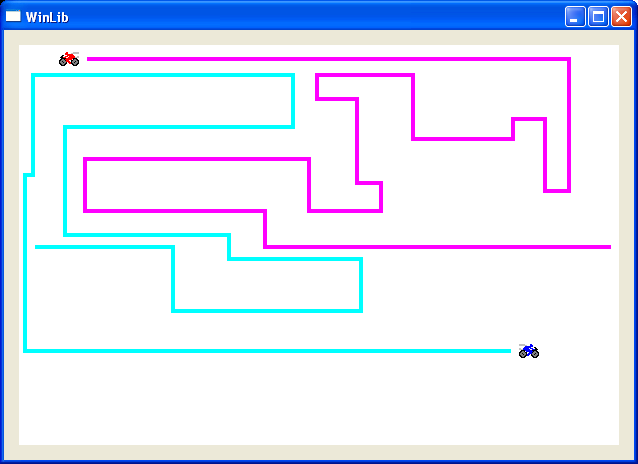
\includegraphics[width=\linewidth]{images/tp.png}
    \end{minipage}
\end{frame}


\end{document}

